\newpage

%% ------------------------------------------------------------
\appendix
%% ------------------------------------------------------------


%% ------------------------------------------------------------
\section{Dataset Construction and Representative Examples}
\label{appendix:dataset}
%% ------------------------------------------------------------
This appendix describes how we built the paired prompt dataset used in the
main experiments. The goal was to keep the agentic scaffold fixed while
changing only the request verb in the user turn.

\subsection{Source Tasks}
\label{appendix:dataset:sources}

We started from programming tasks drawn from APPS, CodeContests, HumanEval,
and MBPP. These sources provide natural code-writing requests with function
signatures, problem statements, examples, tests, or reference solutions. We
used them as task content. The final model input was always rendered into the
same agentic prompt format described in Appendix~\ref{appendix:dataset:template}.

\begin{table}[h]
\centering
\scriptsize
\caption{Raw source-task snapshots used for dataset construction. Counts are
the number of raw records in the local source files before prompt conversion
and behavioral filtering.}
\label{tab:appendix-source-tasks}
\begin{tabularx}{\linewidth}{llr>{\raggedright\arraybackslash}X>{\raggedright\arraybackslash}X}
\toprule
Source & Language(s) used & Raw records & Raw task form & Example raw task \\
\midrule
APPS & Python & 5,000 & Competitive-programming style statements with examples and reference solutions. & Decode a password by subtracting two from each digit. \\
CodeContests & C++, Java & 165 & Contest statements with public tests and submitted solutions. & Sort strings under a custom odd/even character ordering rule. \\
HumanEval & Python & 164 & Python function signatures with docstrings and unit tests. & Check whether two numbers in a list are closer than a threshold. \\
MBPP & Python & 120 & Short Python programming problems with examples and tests. & Return the first repeated character in a string. \\
\bottomrule
\end{tabularx}
\end{table}

These examples show the kind of content we kept from the original datasets:
the programming problem itself, the required function behavior, and any useful
examples or tests. We did not keep the original dataset formatting in the final
prompt. The following boxes show the raw formats before conversion. They are
shortened for readability, but preserve the fields used by our conversion
pipeline. Each task was then converted into the common format described in
Appendix~\ref{appendix:dataset:pipeline}.

\promptboxcaption{APPS raw task format.}
\begin{PromptBox}
{
  "id": 1058,
  "question": "There is a popular app named Exbook ... find the
original password if the portal shows every digit after adding two.

-----Input-----
The first line contains t ...

-----Sample Input-----
2
3527
47269

-----Sample Output-----
1305
25047",
  "solutions": ["for _ in range(int(input())): ..."],
  "input_output": {"inputs": [["2", "3527", "47269"]],
                   "outputs": [["1305", "25047"]]}
}
\end{PromptBox}

\promptboxcaption{CodeContests raw task format.}
\begin{PromptBox}
name: 1575_A. Another Sorting Problem
description: Andi and Budi were given an assignment to tidy up their
bookshelf of n books ... sort it asc-desc-endingly ...
public_tests:
  input:  "5 2\nAA\nAB\nBB\nBA\nAZ\n"
  output: "5 2 1 3 4\n"
solutions:
  language: [C++, Java, ...]
  solution: ["#include <bits/stdc++.h> ...", "import java.io.*; ..."]
\end{PromptBox}

\promptboxcaption{HumanEval raw task format.}
\begin{PromptBox}
task_id: HumanEval/0
prompt:
  def has_close_elements(numbers: List[float], threshold: float) -> bool:
      """Check if any two numbers are closer than the threshold.
      >>> has_close_elements([1.0, 2.0, 3.0], 0.5)
      False
      """
canonical_solution:
  for idx, elem in enumerate(numbers):
      ...
test:
  assert candidate([1.0, 2.0, 3.9, 4.0], 0.3) == True
\end{PromptBox}

\promptboxcaption{MBPP raw task format.}
\begin{PromptBox}
task_id: 602
prompt: Write a python function to find the first repeated character
in a given string.
code:
  def first_repeated_char(str1):
      ...
test_list:
  assert first_repeated_char("abcabc") == "a"
  assert first_repeated_char("abc") == None
\end{PromptBox}

\subsection{Agentic Prompt Template}
\label{appendix:dataset:template}

Each example was rendered with Qwen's official chat template. The tool schema
and tool-call wrapper follow the LangGraph agent interface used in our
experiments. The system turn provides a single available tool,
\texttt{write\_file}, and states the required \texttt{<tool\_call>}
serialization format. The assistant prefix uses the non-thinking completion
form used by Qwen3. The boxed template below shows the structure; braces mark
fields filled by each task.

\promptboxcaption{Agentic prompt template used for all clean and corrupt prompts.}
\begin{PromptBox}
<|im_start|>system
# Tools

You may call one or more functions to assist with the user query.

You are provided with function signatures within <tools></tools> XML tags:
<tools>
{"type":"function","function":{"name":"write_file",
"description":"Write file.",
"parameters":{"type":"object","properties":{"file_path":{"type":"string"},
"content":{"type":"string"}},"required":["file_path","content"]}}}
</tools>

For each function call, return a json object with function name
and arguments within <tool_call></tool_call> XML tags:
<tool_call>
{"name": <function-name>, "arguments": <args-json-object>}
</tool_call><|im_end|>
<|im_start|>user
{REQUEST_VERB} the function body in {TARGET_FILE} based on the function
definition and docstring below:
{TASK_BODY}
<|im_end|>
<|im_start|>assistant
<think>

</think>
\end{PromptBox}

The tool list, tool schema, output format instruction, target file, task body,
and assistant prefix are identical within each pair; the request verb at the
beginning of the user turn is the only change.

\subsection{Pair Construction Pipeline}
\label{appendix:dataset:pipeline}

Dataset construction proceeded in four stages.

\textbf{Task normalization.}
Raw programming tasks vary across sources. APPS and
CodeContests often provide full contest statements, while HumanEval and MBPP
usually provide function signatures and tests. We used ChatGPT-5 to convert
raw tasks into a common function-completion form. The conversion standardizes
the task format; it does not translate a task from one programming language
to another. The converted task keeps the core problem statement, signature,
docstring, and examples when available, and expresses the request as a
completion task for the corresponding file type.

\promptboxcaption{Example instruction used for task normalization.}
\begin{PromptBox}
Convert the following programming problem into a function-completion task.
Keep the original programming language. Keep the function signature, docstring,
examples, and any constraints needed to solve the problem. Do not solve the
problem. Format the result as a prompt asking the assistant to complete the
function body in solve.py, solve.java, or solve.cpp, depending on the original
language.

Input:
[RAW PROGRAMMING TASK HERE]

Output:
<|im_start|>user
Write the function body in {TARGET_FILE} based on the function definition and
docstring below:
{TASK_BODY}
<|im_end|>
\end{PromptBox}

\textbf{Template instantiation.}
Each normalized task was inserted into the agentic template in
Appendix~\ref{appendix:dataset:template}. This step fixes the scaffold and
tool interface before the clean/corrupt verb substitution is applied.

\textbf{Verb screening and assignment.}
We screened request verbs with two criteria. First, the verb had to be a
single token under the Qwen tokenizer, so that the paired prompts remained
token-length aligned. Some natural candidates were rejected at this step
because they split into multiple tokens. Second, the verb had to give a clean
behavioral contrast in the fixed scaffold. Execution verbs should make
\texttt{<tool\_call>} the top-1 first token; analysis verbs should make an
ordinary text token the top-1 first token. The final verb pools were:
\begin{align*}
\mathcal{V}_{\mathrm{exec}} &=
\{\textit{add},\textit{build},\textit{complete},\textit{save},\textit{write}\},\\
\mathcal{V}_{\mathrm{analysis}} &=
\{\textit{discuss},\textit{explore},\textit{inspect},\textit{review},\textit{study}\}.
\end{align*}
For each task, we selected one execution verb and one analysis verb that
passed the multi-model filter below. The screening was task-dependent: for
example, \textit{save} was valid for nearly every task, while \textit{build}
and \textit{complete} were useful only for a smaller subset. Tables
\ref{tab:appendix-exec-screening} and
\ref{tab:appendix-analysis-screening} summarize the verb-screening audit
used during construction. The five verbs shown in bold were selected for the
final paired dataset.

\begin{table}[h]
\centering
\scriptsize
\caption{Execution-verb screening. Entries are the percentage of prompts for
which \texttt{<tool\_call>} was the top-1 first token. Bold column names mark
the verbs retained in the final clean pool.}
\label{tab:appendix-exec-screening}
\resizebox{\linewidth}{!}{%
\begin{tabular}{lrrrrrrrrrr}
\toprule
Model & \textbf{add} & \textbf{build} & \textbf{complete} & create & generate & implement & modify & \textbf{save} & update & \textbf{write} \\
\midrule
Qwen3-0.6B & 81.4 & 69.2 & 74.6 & 55.8 & 48.1 & 70.3 & 43.7 & 91.6 & 46.4 & 83.5 \\
Qwen3-1.7B & 87.9 & 10.1 & 41.4 & 39.5 & 31.7 & 58.2 & 35.6 & 100.0 & 42.3 & 55.3 \\
Qwen3-4B & 94.5 & 59.6 & 14.5 & 47.8 & 38.9 & 73.4 & 40.8 & 100.0 & 51.2 & 90.3 \\
Qwen3-8B & 100.0 & 100.0 & 99.9 & 96.3 & 88.4 & 99.1 & 81.7 & 100.0 & 92.6 & 100.0 \\
Qwen3-14B & 99.7 & 98.8 & 99.1 & 93.5 & 85.9 & 97.4 & 78.6 & 100.0 & 89.8 & 99.6 \\
\bottomrule
\end{tabular}%
}
\end{table}

\begin{table}[h]
\centering
\scriptsize
\caption{Analysis-verb screening. Entries are the percentage of prompts for
which \texttt{<tool\_call>} was the top-1 first token. Lower values are better
for corrupt prompts. Bold column names mark the verbs retained in the final
corrupt pool.}
\label{tab:appendix-analysis-screening}
\resizebox{\linewidth}{!}{%
\begin{tabular}{lrrrrrrrrrr}
\toprule
Model & analyze & assess & compare & \textbf{discuss} & examine & \textbf{explore} & \textbf{inspect} & \textbf{review} & summarize & \textbf{study} \\
\midrule
Qwen3-0.6B & 18.6 & 24.3 & 31.7 & 9.8 & 21.1 & 6.2 & 4.9 & 7.5 & 34.8 & 5.7 \\
Qwen3-1.7B & 27.5 & 33.1 & 42.8 & 12.8 & 18.4 & 0.0 & 0.1 & 0.2 & 38.6 & 0.0 \\
Qwen3-4B & 19.4 & 25.7 & 36.2 & 0.0 & 16.9 & 0.0 & 0.1 & 0.2 & 31.4 & 0.8 \\
Qwen3-8B & 41.2 & 52.7 & 63.8 & 0.0 & 35.5 & 5.5 & 55.9 & 9.6 & 68.2 & 21.1 \\
Qwen3-14B & 38.5 & 49.1 & 60.4 & 1.1 & 33.8 & 3.7 & 42.6 & 7.4 & 65.9 & 17.8 \\
\bottomrule
\end{tabular}%
}
\end{table}

\textbf{Behavioral filtering and split.}
The construction filter used Qwen3-1.7B, Qwen3-4B, and Qwen3-8B. We also
checked Qwen3-0.6B and Qwen3-14B during the verb-screening audit in
Tables~\ref{tab:appendix-exec-screening} and
\ref{tab:appendix-analysis-screening}, but they were not used as hard
retention criteria for the final 1,500 pairs. A pair was retained only if the three construction models predicted
\texttt{<tool\_call>} as the top-1 first token on the execution-verb side and
did not predict \texttt{<tool\_call>} as the top-1 first token on the
analysis-verb side. After filtering, the retained pairs were randomly split
into training and held-out evaluation sets with seed 42.

The screening percentages in Tables~\ref{tab:appendix-exec-screening}
and~\ref{tab:appendix-analysis-screening} are aggregate rates across all
candidate tasks. A verb with a high overall \texttt{<tool\_call>} rate on the
analysis side (such as \textit{inspect} at 55.9\% for Qwen3-8B) is not
excluded from the final corpus: retention operates pair by pair. For a given
task, \textit{inspect} is retained as the analysis verb only if all three
construction models produce a non-\texttt{<tool\_call>} first token for that
specific (task, verb) combination. The 342 retained \textit{inspect} pairs are
those that pass this per-pair filter across all three models.

\subsection{Construction Results}
\label{appendix:dataset:results}

The initial pool contained 1,511 candidate tasks. Eleven tasks were removed
because no valid analysis-verb counterpart was available under the multi-model
filter. The final dataset contains 1,500 paired prompts, split into 1,200
training pairs and 300 held-out pairs.

\begin{table}[h]
\centering
\scriptsize
\caption{Train split composition after filtering.}
\label{tab:appendix-train-summary}
\begin{tabularx}{\linewidth}{llrX}
\toprule
Group & Language(s) used & Pairs & Notes \\
\midrule
All train pairs & -- & 1,200 & Random split with seed 42. \\
APPS & Python & 293 & Python code tasks from the APPS source pool. \\
CodeContests & C++, Java & 811 & CodeContests examples rendered into \texttt{solve.cpp} and \texttt{solve.java}. \\
HumanEval & Python & 29 & Python function-completion tasks with docstrings and tests. \\
MBPP & Python & 67 & Short Python programming tasks with tests. \\
\bottomrule
\end{tabularx}
\end{table}

\begin{table}[h]
\centering
\scriptsize
\caption{Held-out split composition after filtering.}
\label{tab:appendix-test-summary}
\begin{tabularx}{\linewidth}{llrX}
\toprule
Group & Language(s) used & Pairs & Notes \\
\midrule
All held-out pairs & -- & 300 & Random split with seed 42. \\
APPS & Python & 76 & Python code tasks from the APPS source pool. \\
CodeContests & C++, Java & 202 & CodeContests examples rendered into \texttt{solve.cpp} and \texttt{solve.java}. \\
HumanEval & Python & 7 & Python function-completion tasks with docstrings and tests. \\
MBPP & Python & 15 & Short Python programming tasks with tests. \\
\bottomrule
\end{tabularx}
\end{table}

Tables~\ref{tab:appendix-train-summary} and
\ref{tab:appendix-test-summary} report the split-specific composition of the
final dataset. CodeContests provides the C++ and Java examples; APPS,
HumanEval, and MBPP provide the Python examples. The language balance is
similar across splits, with CodeContests dominating because it contributes
both C++ and Java tasks.

\begin{table}[h]
\centering
\small
\caption{Final verb distributions after filtering and random split.}
\label{tab:appendix-verb-distribution}
\begin{tabularx}{\linewidth}{lrr|lrr}
\toprule
Execution verb & Total & Test & Analysis verb & Total & Test \\
\midrule
add & 432 & 86 & discuss & 300 & 60 \\
build & 103 & 20 & explore & 300 & 53 \\
complete & 103 & 20 & inspect & 300 & 54 \\
save & 432 & 87 & review & 300 & 60 \\
write & 430 & 87 & study & 300 & 73 \\
\bottomrule
\end{tabularx}
\end{table}

Table~\ref{tab:appendix-verb-distribution} reports the selected verbs after
filtering. The clean side is intentionally not uniform across verbs because
the selection is constrained by the multi-model behavior check. The corrupt
side is close to balanced across the five analysis verbs.

The filtering result was exact for the three construction models:
Qwen3-1.7B, Qwen3-4B, and Qwen3-8B predicted \texttt{<tool\_call>} on all
1,500 clean prompts and predicted a non-\texttt{<tool\_call>} token on all
1,500 corrupt prompts. This filtering step is part of dataset construction,
not a claim about unseen models.

\subsection{A Representative Clean/Corrupt Prompt Pair}
\label{appendix:dataset:example}

The following pair shows the full prompt for one retained Python example.
The system turn, tool schema, task body, and assistant prefix are identical.
Only the first word of the user turn changes.

\promptboxcaption{Representative clean prompt.}
\begin{PromptBox}
<|im_start|>system
# Tools

You may call one or more functions to assist with the user query.

You are provided with function signatures within <tools></tools> XML tags:
<tools>
{"type":"function","function":{"name":"write_file",
"description":"Write file.",
"parameters":{"type":"object","properties":{"file_path":{"type":"string"},
"content":{"type":"string"}},"required":["file_path","content"]}}}
</tools>

For each function call, return a json object with function name
and arguments within <tool_call></tool_call> XML tags:
<tool_call>
{"name": <function-name>, "arguments": <args-json-object>}
</tool_call><|im_end|>
<|im_start|>user
Write the function body in solve.py based on the function definition and
docstring below:
def spinning_rings(inner_max, outer_max):
    """
    Two numbered rings rotate one step in opposite directions from 0 until
    the numbers at the top match again. Return the number of moves needed.
    >>> spinning_rings(2, 3)
    5
    """
    pass
<|im_end|>
<|im_start|>assistant
<think>

</think>
\end{PromptBox}

\promptboxcaption{Representative corrupt prompt paired with the clean prompt above.}
\begin{PromptBox}
<|im_start|>system
# Tools

You may call one or more functions to assist with the user query.

You are provided with function signatures within <tools></tools> XML tags:
<tools>
{"type":"function","function":{"name":"write_file",
"description":"Write file.",
"parameters":{"type":"object","properties":{"file_path":{"type":"string"},
"content":{"type":"string"}},"required":["file_path","content"]}}}
</tools>

For each function call, return a json object with function name
and arguments within <tool_call></tool_call> XML tags:
<tool_call>
{"name": <function-name>, "arguments": <args-json-object>}
</tool_call><|im_end|>
<|im_start|>user
Inspect the function body in solve.py based on the function definition and
docstring below:
def spinning_rings(inner_max, outer_max):
    """
    Two numbered rings rotate one step in opposite directions from 0 until
    the numbers at the top match again. Return the number of moves needed.
    >>> spinning_rings(2, 3)
    5
    """
    pass
<|im_end|>
<|im_start|>assistant
<think>

</think>
\end{PromptBox}

%% ------------------------------------------------------------
\section{Circuit Search: Methods and Failure}
\label{appendix:circuit}
%% ------------------------------------------------------------
Before settling on the representation-level analysis in the main text, we
applied three sparse-circuit search methods to the tool-call decision task:
ACDC, EAP-IG, and Circuit Tracing. Each method identifies circuit components
relevant to a chosen task metric, using different strategies for edge selection
and scoring. This appendix describes each method, presents the task-specific
diagnostic result, and explains why none of the three produced a compact
faithful circuit for this task. All three methods fail for the same structural reason, described in
Appendix~\ref{appendix:circuit:failure}.

\subsection{ACDC}
\label{appendix:circuit:acdc}
ACDC \citep{conmy2023acdc} frames circuit discovery as a pruning problem.
Starting from a large computational graph, it repeatedly tests whether an edge
can be removed while preserving a task metric under activation patching.
Edges whose removal changes the metric beyond a chosen threshold are retained;
the intended output is a small subgraph whose retained edges are sufficient
for the behavior and whose removal is necessary for the behavior.

For the tool-call task we apply the same faithfulness logic to clean/corrupt
prompt pairs.
Sufficiency asks whether the ACDC circuit, run with non-circuit computation
corrupted or ablated, still restores the clean \texttt{<tool\_call>} decision.
Necessity asks whether removing the discovered circuit from the clean run
suppresses the \texttt{<tool\_call>} decision.
Table~\ref{tab:appendix-acdc-faithfulness} reports the faithfulness results
for the archived sparse forward-core replay runs that were produced during the
earlier ACDC-style search stage.

\begin{table}[h]
  \centering
  \small
  \caption{Archived sparse forward-core replay summary across Qwen3 scales.
  Core nodes and edges are taken from the aggregated forward sparse graph.
  Suff.\ is the mean replay ratio of the discovered core relative to the clean
  baseline, Necc.\ is the mean ratio under clean-run removal, Rand.\ Suff.\ is
  the mean replay ratio of size-matched random cores, and Gap is the mean
  advantage of the discovered core over the random baseline. These archived
  ratios are reported for completeness only; they are not the final causal
  metrics used in the main text.}
  \label{tab:appendix-acdc-faithfulness}
  \begin{tabular}{lcccccc}
  \toprule
  Model & Core nodes & Core edges & Suff. & Necc. & Rand.\ Suff. & Gap \\
  \midrule
  Qwen3-1.7B & 18 & 54 & 0.9891 & 0.9824 & 0.8812 & 0.1078 \\
  Qwen3-4B & 18 & 69 & 0.9979 & 0.8319 & 0.8712 & 0.1266 \\
  Qwen3-8B & 18 & 63 & 1.0000 & 0.5975 & 0.9768 & 0.0232 \\
  Qwen3-14B & 20 & 86 & 0.9999 & 0.4077 & 0.9554 & 0.0446 \\
  \bottomrule
\end{tabular}
\end{table}

The archived replay ratios already show the problem. The sparse graphs are
large, and the advantage over size-matched random cores becomes small at 8B
and 14B even when sufficiency stays near 1.0. Necessity also weakens as model
size grows. The sparse graph highlights the relevant regions; the localized tool-call
vector identified in the main text remains the decisive causal object.

\subsection{EAP-IG}
\label{appendix:circuit:eap}
EAP-IG \citep{syed2023attribution} replaces repeated causal edge patching with
a scalable attribution score.
For each edge, it estimates the effect of changing the edge activation between
clean and corrupt runs; integrated gradients are used to avoid relying only on
the local gradient at one endpoint.
Edges are then ranked by score, and a circuit is obtained by taking the
highest-scoring edges or by greedily adding high-scoring edges that connect to
the current subgraph.
The relevant standard is faithfulness: after non-circuit edges are corrupted,
the retained circuit should still reproduce the original task behavior
\citep{hanna2024faithfulness}.

\begin{figure}[h]
  \centering
  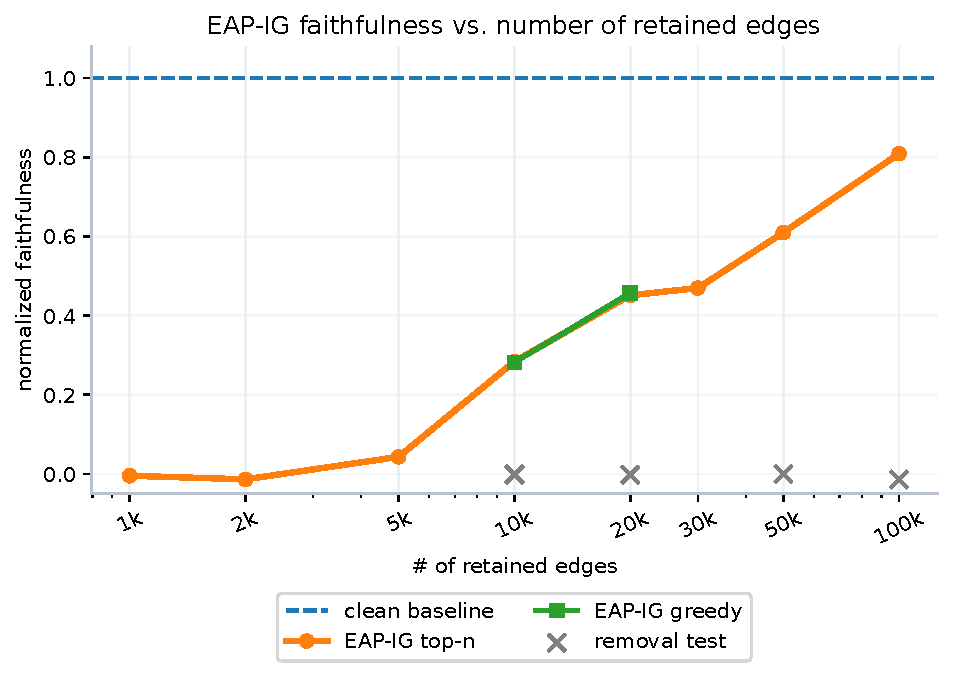
\includegraphics[width=0.78\linewidth]{figures/appendix_eap_ig_faithfulness.pdf}
  \caption{EAP-IG top-$k$ faithfulness curve for the tool-call task, normalized
  between the corrupt and clean baselines. Faithful recovery of the
  \texttt{<tool\_call>} signal requires a very large retained edge set,
  confirming that no compact sparse circuit accounts for the behavior.}
  \label{fig:appendix-eap-ig-faithfulness}
\end{figure}

\begin{table}[h]
  \centering
  \small
  \caption{EAP-IG top-$k$ sweep on Qwen3-8B using 100 equal-length clean/corrupt
  prompt pairs. Faith.\ normalizes sufficiency between the corrupt and clean
  baselines. Suff.\ is the mean logit-difference score under corrupt-side
  replay with only the retained edges active; Removal is the corresponding
  score after removing the retained edges from the clean run when evaluated.
  Nodes counts the retained component set induced by the edges.}
  \label{tab:appendix-eap-ig-topk}
  \begin{tabular}{lrrrrr}
  \toprule
  Retained edges & Faith. & Suff. logit diff & Removal logit diff & Nodes & Core overlap \\
  \midrule
  1,000 & -0.005 & -13.12 &  & 139 & 17/18 \\
  2,000 & -0.014 & -13.38 &  & 229 & 18/18 \\
  5,000 & 0.043 & -11.81 &  & 417 & 18/18 \\
  10,000 & 0.284 & -5.19 & -13.06 & 553 & 18/18 \\
  20,000 & 0.451 & -0.59 &  & 708 & 18/18 \\
  30,000 & 0.470 & -0.08 &  & 805 & 18/18 \\
  50,000 & 0.610 & 3.77 & -13.00 & 937 & 18/18 \\
  100,000 & 0.809 & 9.25 & -13.38 & 1075 & 18/18 \\
  \bottomrule
\end{tabular}
\end{table}

On the tool-call task, the 8B EAP-IG sweep shows the same qualitative issue.
On a 100-pair run, top-$10$k edges still leaves the mean sufficiency score at
$-5.19$, far below the clean baseline. Top-$50$k edges raises that score to
$3.77$, but this requires 937 retained nodes and is still far from the clean
baseline of $14.50$. A supplemental top-$100$k point reaches $9.25$, but only
after retaining 1,075 induced nodes. The retained node set fully overlaps with
the 18-node heuristic forward core from top-$2$k onward, so the problem is not
missed components. The problem is that faithful recovery requires a very large
edge set. The edge ranking therefore recovers many relevant components, but the
tool-call decision is carried by a dense direction in the prediction-position
residual state, not by a compact set of edge paths.

\subsection{Circuit Tracing}
\label{appendix:circuit:tracing}
Circuit Tracing \citep{anthropic2025circuit} operates below the level of whole
heads and whole MLP blocks. In our use case, it builds a prompt-specific local
graph in which attention patterns and normalization terms are treated as fixed,
while the MLP updates are expanded into sparse feature contributions. The graph
then supports direct-effect measurements between feature activations,
attention-mediated transfers, reconstruction-error terms, and the output logits.
Appendix~\ref{appendix:transcoder} provides the separate feature analysis that
we use for the formation-window claims in the main text.

For this task, the method is most useful as a local diagnostic rather than as a
compact end-to-end circuit finder. It shows that multiple formation-window
features fire more strongly on analysis prompts and push against
$\hat{\mu}_\Delta$, which is exactly the semantic evidence needed for the
suppressor account. The difficulty appears when we ask for one pruned graph that
links the verb token, the long scaffold, the formation-window features, the
downstream readers, and the final \texttt{<tool\_call>} logit. Even after
pruning, the traced graph remains broad rather than collapsing into a narrow
route. Figure~\ref{fig:appendix-feature-circuit} shows a representative
pruned circuit for one clean prompt: even after aggressive edge pruning, the
graph contains hundreds of feature-to-feature connections, confirming that the
relevant signal cannot be captured by a small routing subgraph. The reason is
the same one seen with the other circuit-search methods:
the relevant information is distributed across a long prompt scaffold and is
best summarized by the dense prediction-position state, not by a tiny
feature-to-feature chain.

\begin{figure}[h]
  \centering
  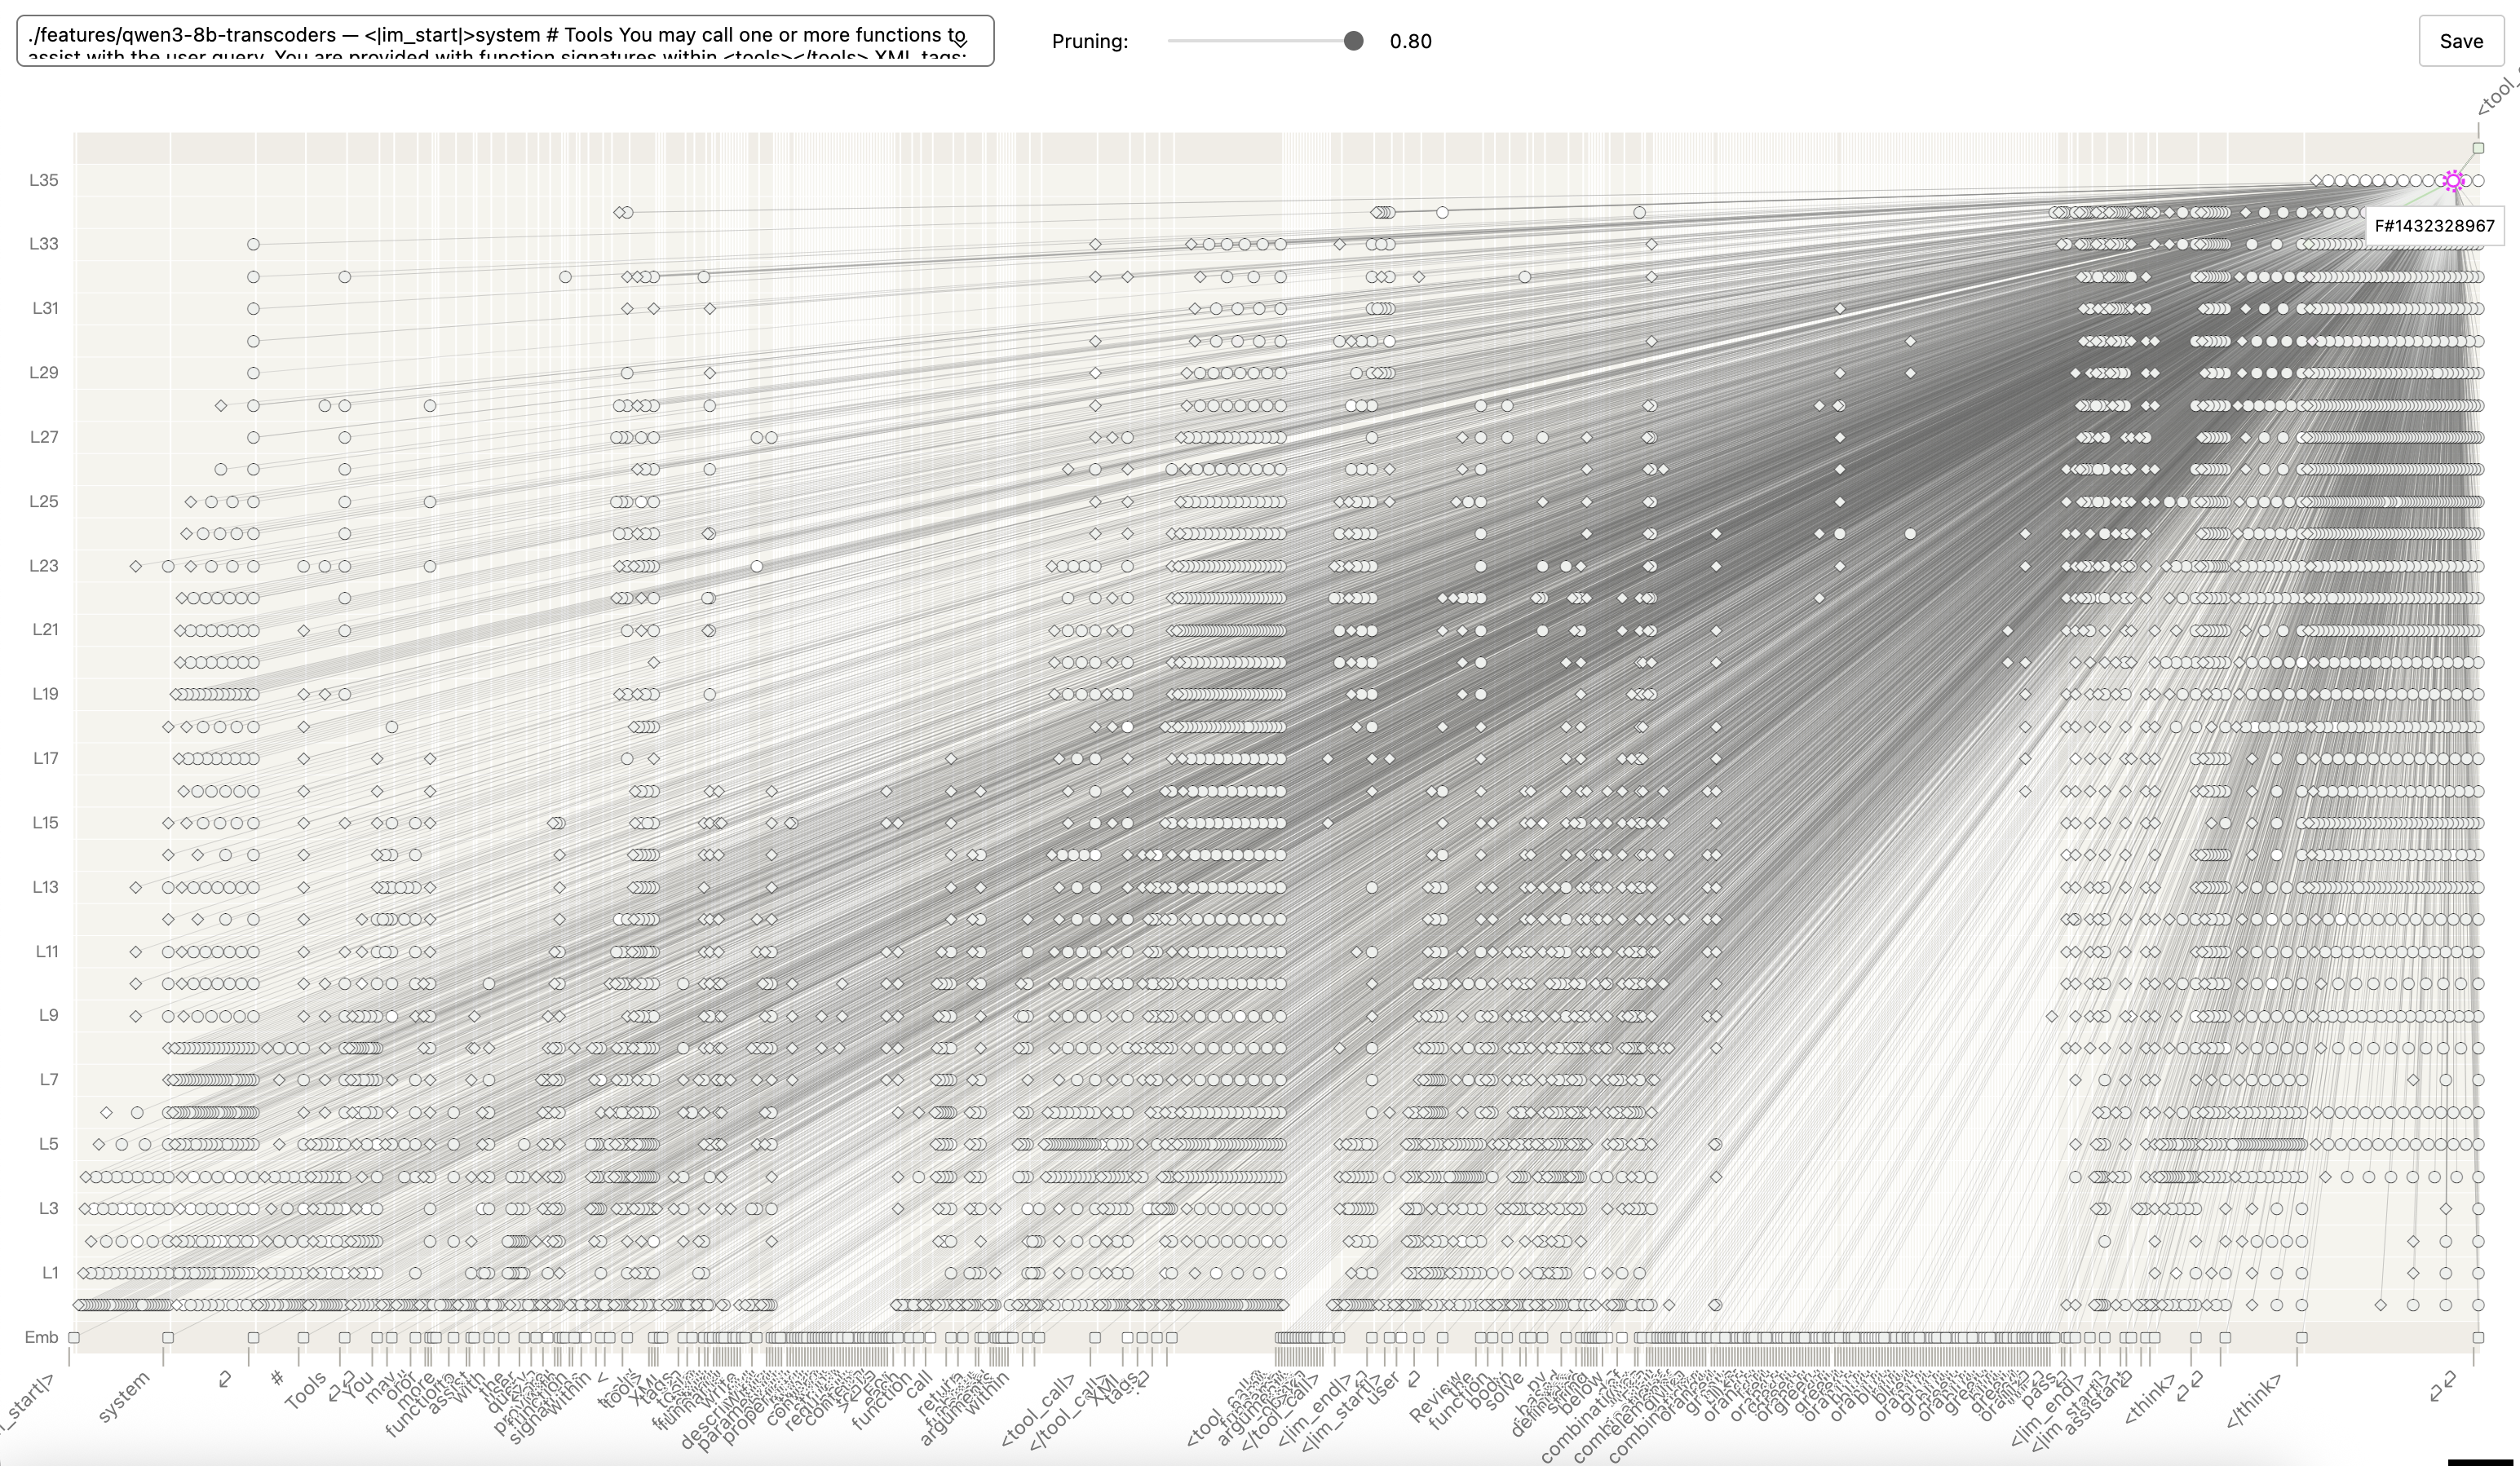
\includegraphics[width=\linewidth]{figures/feature_circuit.png}
  \caption{Feature circuit graph produced by Circuit Tracing \citep{anthropic2025circuit}
  for one representative clean prompt at the default pruning threshold.
  Each node is a transcoder feature or residual-stream component; edges carry
  direct-effect attribution weight. The graph remains broad and densely
  connected after pruning, illustrating why the circuit-search approach cannot
  isolate a compact subgraph: the call-or-no-call signal is distributed across
  the full prompt scaffold and aggregates into a dense prediction-position direction
  rather than flowing through a narrow feature-to-feature chain.}
  \label{fig:appendix-feature-circuit}
\end{figure}

\subsection{Why Circuit Search Methods Fail Here}
\label{appendix:circuit:failure}
All three methods share the same underlying assumption: that the decision is
mediated by a sparse, identifiable subgraph of edges or feature pairs.
This assumption fails in the tool-call setting for a structural reason.
The agentic scaffold spans several hundred tokens; the call-or-no-call signal
must integrate verb semantics from the user-turn position with the formatting
bias accumulated from the system turn.
This integration accumulates gradually across layers and positions into a
dense residual-stream direction at layer~24, without passing through any
identifiable small routing subgraph.
A sparse circuit can only capture this process by including the full
prediction-position residual state at layer~24 as a node, at which point the
``circuit'' reduces to the (layer,~position) coordinate identified by
activation patching, and the graph adds nothing beyond the activation-patching result.

The failure is structural, not method-specific: when a binary decision is
governed by a dense directional signal in a long-context scaffold, circuit
search cannot improve on activation patching, and the appropriate granularity
shifts from the edge (circuit level) to the direction (representation level).
We therefore adopt the following approach in the main text: localize the signal to
(layer~24, prediction position) via activation patching, characterize the
direction $\mu_\Delta$ and its causal necessity and sufficiency, and then
decompose the writes into that direction using transcoder feature scores,
bypassing the between-layer routing problem entirely.

%% ------------------------------------------------------------
\section{Transcoder: Method and Full Feature Analysis}
\label{appendix:transcoder}
%% ------------------------------------------------------------
This appendix gives the feature-level view of the formation window.
The main question is simple: once the localized tool-call direction
$\mu_\Delta$ is fixed, which MLP features write into it, and what do those
features mean in ordinary language?

\subsection{What a Transcoder Is}
Instead of treating an MLP update as one opaque residual-stream vector, we
rewrite it in a sparse feature basis. For an MLP input activation
$h \in \mathbb{R}^d$, the auxiliary model computes feature activations
\[
  z = f(W_{\mathrm{enc}} h + b_{\mathrm{enc}}),
\]
and then uses them to approximate the block output:
\[
  \tilde{h}' = W_{\mathrm{dec}} z + b_{\mathrm{dec}}.
\]
The coordinates of $z$ are the units we inspect. Because only a small subset is
active on any one prompt, the decomposition lets us separate two questions that
are otherwise entangled in a dense MLP write: which contexts turn a feature on,
and what direction that feature contributes to the residual stream. For the
present appendix, the practical value is that the formation-window write can be
broken into individually readable pieces rather than treated as a single vector.

For the formation window we use the Qwen3-8B transcoder checkpoints for
L20--L23. Those are the layers where the vector write becomes concentrated in
the main text. The feature analysis is therefore local to the same window,
with the same held-out 300 pairs.

\subsection{How We Score Features}
For each feature $f$ in layer $\ell$, we compute a vector-alignment score
\[
  \kappa_{\ell f}
  = (\bar{a}^c_{\ell f} - \bar{a}^*_{\ell f})
    \langle w_f^{(\ell)}, \hat{\mu}_\Delta \rangle,
\]
where $\bar{a}^c_{\ell f}$ and $\bar{a}^*_{\ell f}$ are the mean clean and
corrupt activations on the held-out pairs.
The inner product term measures whether the decoder direction points toward
or away from the tool-call vector direction. This product combines the sign
and magnitude of the effect.

The sign of $\kappa$ says whether the feature supports the clean-minus-corrupt
tool-call gap. Positive $\kappa$ has two possible sources. A feature can be
higher on clean prompts and write toward the tool-call vector, or it can be
higher on corrupt prompts and write away from the tool-call vector. Negative
$\kappa$ marks the two opposite cases. We therefore read each feature using
both terms in the product: the activation difference tells us which prompt side
activates the feature more, and the decoder projection tells us what direction
the feature writes.
We also record the mean activation difference, the decoder projection, and
the top and bottom unembedding tokens for each feature.
Layer-level summaries use
\[
K_{\mathrm{corrupt}}^{(\ell)}
= \sum_{f:\bar{a}^*_{\ell f}>\bar{a}^c_{\ell f}} |\kappa_{\ell f}|,
\qquad
K_{\mathrm{clean}}^{(\ell)}
= \sum_{f:\bar{a}^c_{\ell f}>\bar{a}^*_{\ell f}} |\kappa_{\ell f}|.
\]
These totals group features by which prompt side activates them more strongly.
They keep the activation-side question separate from the sign of $\kappa$.

\subsection{How We Read the Features}
We do not assign labels from $\kappa$ alone. A feature name is chosen only
after combining three kinds of evidence: the prompts on which the feature peaks,
the vocabulary items most strongly favored or disfavored by its decoder
direction, and the sign pattern given by the activation difference together with
the projection onto $\hat{\mu}_\Delta$. That combination lets us tell apart,
for example, a feature that rises on analysis prompts and suppresses the
tool-call state from one that rises on clean prompts and reinforces it. The
labels in this appendix are therefore short summaries of the dominant behavior,
not claims that a feature responds to only one exact phrase.

\begin{figure}[t]
  \centering
  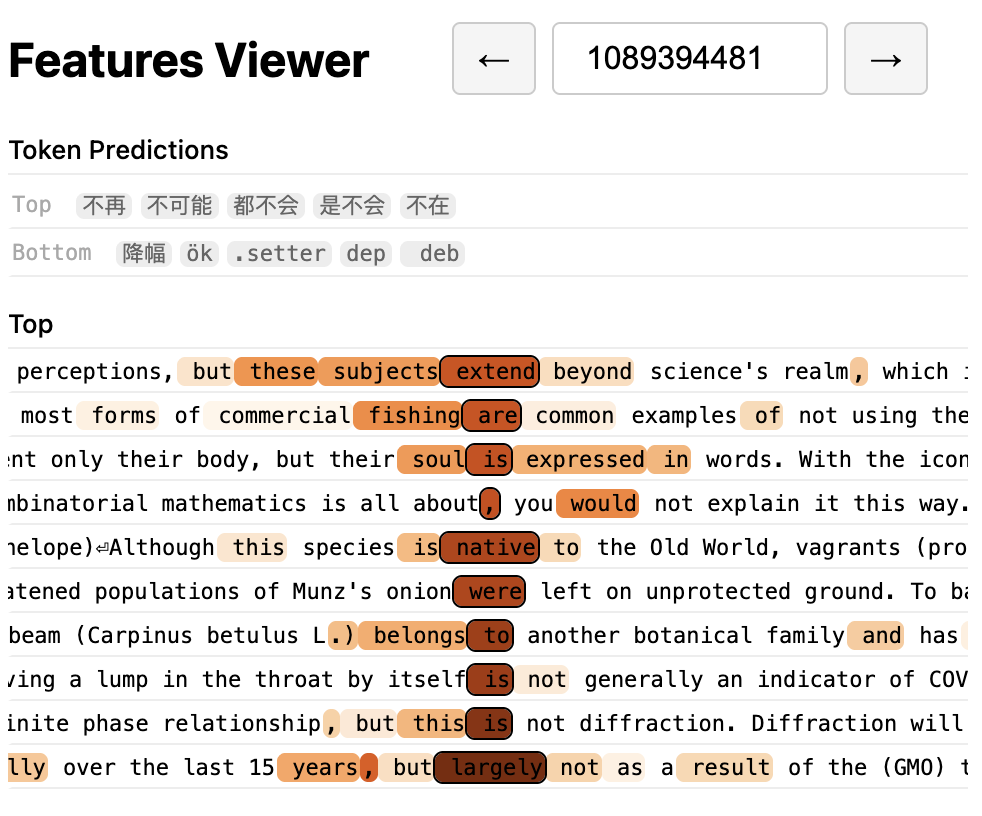
\includegraphics[width=\linewidth]{figures/feature1.png}
  \caption{A representative formation-window transcoder feature displayed in
  the Features Viewer. The top panel shows token-level activation highlighting
  across a max-activating context: darker or colored tokens are those that most
  strongly activate the feature. The two prediction rows (Top / Bottom) give
  the vocabulary tokens most favored and disfavored by the feature's decoder
  direction $w_f^{(\ell)}$. This feature belongs to the
  \texttt{analysis\_non\_execution} family: it fires on analysis-verb contexts
  (e.g.\ \textit{discuss}, \textit{review}) and its decoder direction writes
  away from $\hat{\mu}_\Delta$, suppressing the tool-call state on corrupt prompts.}
  \label{fig:appendix-feature-gallery}
\end{figure}

\subsection{Feature Families in the Formation Window}
The scored features cluster into a small number of recurring families.
Table~\ref{tab:appendix-transcoder-families} gives the compact summary used in
the paper.

\begin{table}[h]
\centering
\small
  \caption{Formation-window transcoder families ranked by $|\kappa|$ mass. The
family label is assigned from the max-activating prompts and decoder tokens,
not from the score alone. The side column records whether the family contributes
mainly to $K_{\mathrm{corrupt}}$ or $K_{\mathrm{clean}}$.}
\label{tab:appendix-transcoder-families}
\begin{tabularx}{\linewidth}{lccccX}
\toprule
Family & Side & Layers & Members & Total $|\kappa|$ & Readable label \\
\midrule
  \texttt{analysis\_non\_execution} & corrupt & L20--L23 & 43 & 23.1828 & analysis verbs, no need, non-existence \\
  \texttt{execution\_request} & clean & L20--L23 & 77 & 12.3622 & execution requests and action verbs \\
  \texttt{analysis\_plain\_discourse} & corrupt & L20--L23 & 16 & 4.1119 & plain analysis discourse \\
  \texttt{schema\_boundary\_formatting} & clean & L20--L23 & 14 & 1.7315 & code and format boundaries \\
\bottomrule
\end{tabularx}
\end{table}

The strongest family is \texttt{analysis\_non\_execution}. Its members are
concentrated in L21--L23, and most of them write away from the tool-call
vector on corrupt prompts. The clean-side \texttt{execution\_request} family
also contributes, but with smaller $|\kappa|$ mass overall. This matches the
main text: $K_{\mathrm{corrupt}}$ exceeds $K_{\mathrm{clean}}$ in L21--L23,
so the largest feature-level contribution comes from corrupt-side suppressor
features rather than clean-side execution features.

\subsection{Representative Examples}
The feature labels are easiest to see in the held-out prompt examples.
Features in the analysis family tend to activate on words like
\textit{discuss}, \textit{study}, \textit{review}, \textit{explore}, and
\textit{inspect}, along with contexts that imply no tool is needed.
The clean-side family instead lights up on action verbs such as
\textit{write}, \textit{build}, \textit{complete}, \textit{save}, and
\textit{add}.

The downstream token views are also simple to read.
Boundary and serialization features place mass on code punctuation, line
breaks, and formatting markers.
Those features are useful in the late readout window, but in the formation
window the dominant contribution is still semantic: whether the prompt requests
an action or analysis.

\subsection{Causal Ablation}
The family labels matter only if they survive causal intervention.
Ablating the top five \texttt{analysis\_non\_execution} feature activations on the
held-out corrupt prompts shifts the mean layer-24 vector-score by $-27.4550$,
and 47.93\% of corrupt prompts flip to \texttt{<tool\_call>} top-1.
A matched random control shifts the vector score by only $0.2788$ on average
across eight seeds.

The same family also behaves consistently under patching: clean- and corrupt-side
activation swaps move the vector score in the expected direction, and the effect
stays centered on the layer-24 vector state, with no sign of a separate bypass path.

\subsection{Formation Mediation}
Patching only the four formation-window MLPs (L20--L23) from clean into the
corrupt forward pass recovers \texttt{<tool\_call>} top-1 on 93.89\% of corrupt
prompts; restoring only the $\hat{\mu}_\Delta$-aligned component at layer~24
then closes 100\% of the lost vector-state gap and brings top-1 back to 100\%.
The formation-window MLP contribution to the decision flows entirely through the
$\hat{\mu}_\Delta$ direction, with no evidence of a separate bypass path.

The late-layer feature analysis is kept with the downstream readout appendix
(Appendix~\ref{appendix:readout}) because it addresses a separate question:
how the already-formed vector is translated into output structure.

%% ------------------------------------------------------------
\section{Downstream Readout: Full Evidence}
\label{appendix:readout}
%% ------------------------------------------------------------
This appendix gives the full evidence behind the downstream-readout claim in
Section~\ref{sec:readout}. Section~\ref{sec:vector-state} established that a
compact tool-call vector exists at layer~24; the question here is what
downstream components do with that state once it is present.  We therefore restrict the primary sweep to layers~25--35, which are
strictly downstream of the L24 decision state, and evaluate every component on
the same 300 held-out prompt pairs used in the main text.

Across the experiments below, the evidence supports three conclusions. First,
readout is distributed: no single downstream attention head is a faithful
bottleneck, although several heads are reliable readers of the layer-24
tool-call vector. Second, the readout components fall into two groups: bridge
heads in L25--L29 that primarily redistribute attention over scaffold regions,
and late attention heads and MLP blocks in L33--L35 that carry the largest
direct output writes. Third, the late MLP write is structurally interpretable:
the most localized feature-level evidence points to a boundary/serialization
family that opens the tool-call format, separately from the semantic decision
encoded in the tool-call vector.

\subsection{DLA Sweep Methodology and Full Rankings (L25--L35)}
For each downstream attention head and MLP block, we measure two quantities.
The first is the clean-minus-corrupt DLA delta for the
\texttt{<tool\_call>} logit.  This asks whether the component writes more
toward the tool-call token when the tool-call vector is present.  The second
is a single-component patching score.  For a component $m$, we replace its
corrupt-side output with the clean-side output at the same layer and position,
then record both the mean \texttt{<tool\_call>} logit shift and the strict
flip rate.  We also run the reverse intervention on clean prompts and record
the corresponding logit drop.  We rank by flip rate with DLA as a tie-breaker, so that a component with a
large logit effect but negligible output attribution is not ranked as the
main reader.

Table~\ref{tab:appendix-readout-heads} reports the top downstream attention
heads.  The ranking separates two roles.  L25--L29 heads usually have modest
DLA but high single-head recovery: they are bridge readers whose patched
outputs help re-establish the downstream state.  L33 heads have much larger
DLA deltas: they are closer to the final output implementation, although a
single L33 head alone is still far from sufficient.

\begin{table}[t]
  \centering
  \small
  \caption{Top downstream attention heads in the L25--L35 sweep on 300
  held-out pairs.  DLA delta is clean minus corrupt for the
  \texttt{<tool\_call>} logit.  Recovery shift and strict flip are measured by
  replacing the corrupt-side head output with the clean-side output.}
  \label{tab:appendix-readout-heads}
  \begin{tabular}{llrrrr}
    \toprule
    Head & role & DLA $\Delta$ & recover shift & corrupt top-1 & strict flip \\
    \midrule
    L29H9  & bridge & 4.15 & 1.34 & 21.3\% & 17.8\% \\
    L33H29 & late implementation & 7.91 & 0.62 & 8.5\% & 4.9\% \\
    L28H3  & bridge & 0.26 & 1.38 & 36.1\% & 32.5\% \\
    L25H6  & bridge & 0.06 & 1.28 & 40.4\% & 36.9\% \\
    L26H14 & bridge & 0.04 & 0.91 & 24.3\% & 20.7\% \\
    L33H11 & late implementation & 3.32 & -0.39 & 2.4\% & 0.0\% \\
    \bottomrule
  \end{tabular}
\end{table}

The MLP sweep is more concentrated (Table~\ref{tab:appendix-readout-mlps}).
MLP34 is the strongest single downstream MLP by the combined score, with a
mean recovery shift of 1.74, a reverse-direction logit drop of 2.32, and a
strict corrupt-side flip rate of 49.7\%.  MLP25 and MLP27 also have large
single-block recovery rates, consistent with a distributed readout stack
rather than a single final-layer formatting block.

\begin{table}[t]
  \centering
  \small
  \caption{Top downstream MLP blocks in the L25--L35 sweep.  Each row patches
  only one MLP output from clean into corrupt, or from corrupt into clean for
  the reverse drop measurement.}
  \label{tab:appendix-readout-mlps}
  \begin{tabular}{lrrrr}
    \toprule
    MLP & recover shift & drop shift & corrupt top-1 & strict flip \\
    \midrule
    L34 & 1.74 & 2.32 & 53.3\% & 49.7\% \\
    L25 & 1.70 & 0.96 & 44.8\% & 41.2\% \\
    L27 & 1.32 & 0.82 & 52.3\% & 48.7\% \\
    L35 & 0.84 & 1.27 & 31.8\% & 28.2\% \\
    L29 & 0.38 & 1.58 & 26.6\% & 23.1\% \\
    L31 & 0.90 & 0.90 & 28.6\% & 25.0\% \\
    \bottomrule
  \end{tabular}
\end{table}

\subsection{Top-4 Attention Head Detailed Analyses}
The top heads differ in how they read the L24 vector.  We label a head as a
bridge head when its clean/corrupt attention difference is concentrated on
remote scaffold regions rather than on the immediate suffix.  We label it as a
late implementation head when it sits in the final third of the model and has
substantial DLA mass at the prediction-adjacent readout stage.

L29H9 is the clearest bridge head.  Its dominant clean-minus-corrupt attention
shift is on the tool-schema region ($+52.9$ percentage points),
while attention to verb, task-description, and suffix regions decreases.  The corresponding
QK diagnostics show that this is not a small local perturbation: the schema,
verb, and suffix QK deltas are 3.41, 17.04, and 10.72, respectively.  Its
query direction remains stable across clean and corrupt prompts
(mean cosine 0.924), suggesting that the main difference is which scaffold
keys become available to the head under the tool-call state.

L28H3 is another bridge reader but with weaker DLA.  It has one of the largest
behavioral single-head effects in the sweep (32.5\% strict corrupt flips) and
a system-region attention increase of $49.5$ percentage points, but its DLA
delta is only 0.26.  This is the characteristic signature of a bridge reader:
patching it helps put later readers into the right state, but the head itself
does not directly carry much of the final \texttt{<tool\_call>} logit.

L33H29 and L33H11 are late implementation heads.  L33H29 has the largest
attention-head DLA delta in the sweep ($+7.91$) and recovers from a corrupt
DLA baseline of 16.85 to 24.67 under L24 state restoration.  L33H11 has a
smaller but still substantial DLA delta ($+3.32$) and restores from 2.36 to
5.46 under the same vector-addition condition.  These heads are therefore best
described as late readers of the L24 state, not as the state itself.

The vector-centered dependence test makes this distinction explicit. Restoring
the full layer-24 tool-call vector gives the late implementation heads a mean
DLA restoration ratio of 0.958 and reaches a best corrupt strict flip rate of
96.45\%. In contrast, patching only the bridge head L29H9 gives a mean DLA
restoration ratio of $-0.141$. The late implementation heads are therefore
downstream of the layer-24 vector, while no single bridge head is the sole
relay between the vector state and the output.

\subsection{MLP34 Structural Feature Family: F109925 and Neighbors}
MLP34 is the most interpretable late writer because its output can be decomposed
at feature resolution.  The main-text analysis identifies L34~F109925 as the
dominant structural feature: it fires on tool-schema boundary contexts,
including \texttt{<tools>}\textbackslash\texttt{n} and nearby
\texttt{function}-schema tokens, and writes toward the
\texttt{<tool\_call>} opening.  Its projected tool-call write is 88.4 in clean
prompts, 48.4 in corrupt prompts, and 87.3 after adding $\mu_\Delta$ back to
corrupt prompts at L24.  A norm-matched random direction leaves the feature
near its corrupt baseline, ruling out a confound from raw activation magnitude.

The causal feature intervention is deliberately local.  We do not patch MLP34
as a block; instead, we replace only the corrupt-side activation scalar of the
selected feature with its clean-side scalar while keeping all other late
features fixed.  Replacing F109925 alone recovers \texttt{<tool\_call>} top-1
on 83.2\% of held-out corrupt prompts, compared with 30.2\% for a matched
non-structural control.  Extending the intervention to the top-5
boundary-support family raises recovery to 92.3\%, compared with 51.1\% for
the matched control family.  This feature-level result is why we describe the
late MLP stage as a semantic-to-structural translation: the tool-call vector
carries whether a call should be made, while the late features implement the
opening format used to begin the call.

The neighboring late features have the same broad semantics.  The late-feature
summary is dominated by code-syntax, code-structure, and serialization labels:
for example L35~F12174, L35~F73574, L35~F134127, L35~F53486, and
L34~F120915 are all clean-higher serialization features, with clean/corrupt
activation ratios ranging from 0.28 to 0.71.  F109925 itself is clean-higher
on all held-out prompts in this analysis.  These neighbors support the same
interpretation but are not individually claimed as the unique causal mechanism;
the faithful intervention is the F109925 and top-5-family result above.

\subsection{Alternative Downstream Path Controls}
Two controls rule out the simplest serial-path explanations. First, ablating
the bridge heads does not erase the late DLA. After zeroing the selected bridge
heads (L29H9, L28H3, L29H11, L26H14, and L29H14), L33H29 retains 97.8\% of
its DLA, L33H11 retains 80.4\%, and MLP34 retains 67.0\%. Behavior is also
almost unchanged: clean top-1 remains 99.8\%. The model substantially drops
\texttt{<tool\_call>} top-1 only when both the bridge heads and the late
attention heads and MLP blocks are removed together, falling to 32.5\%. This is
inconsistent with a strict bridge-to-writer chain in which late writers depend
entirely on the bridge heads.

Second, removing the L24 tool-call vector directly reduces late-layer DLA mass.
On clean prompts, subtracting $\mu_\Delta$ at L24 drops top-1 from 100.0\% to
1.78\%
and removes 35.45\% of the total L30--L35 DLA.  The largest absolute drops are
in L34 (19.46), L33 (16.28), and L35 (15.93), with layer-level drop fractions
of 43.0\%, 39.9\%, and 26.3\%, respectively.  This shows that the late writers
are causally downstream of the L24 vector rather than merely correlated with
the clean condition.

Finally, group ablations confirm the distributed nature of readout.  Zeroing
single readout modules has little effect on clean top-1, but it reduces the
tool-call logit by different amounts: 1.02 for L29H9, 0.47 for L28H3, 0.44
for L33H29, 0.24 for L33H11, 2.33 for MLP34, and 0.96 for MLP25.  Combining
the bridge heads with the late heads and MLPs gives a 5.02 logit drop,
a combined effect 2.16 times larger than the best single-module result.  The strict top-1 drop
under this combined intervention is still only 0.99\%, because the clean
condition has substantial residual margin, but the logit evidence is clear:
readout is carried by a redundant set of downstream writers rather than by a
single fragile component.

%% ------------------------------------------------------------
\section{Early-Layer Signals and Suppression Hypotheses}
\label{appendix:early-layer}
%% ------------------------------------------------------------
This appendix separates three things that are easy to conflate: early linear
recoverability, the layer at which the decision becomes causally committed,
and the feature family that best explains the suppressor signal that forms the
layer-24 tool-call vector.

\subsection{Early Separability vs.\ Late Causal Commitment}
On 300 held-out pairs, the probe already reaches AUC $> 0.9$ at L1, so the
clean/corrupt distinction is linearly recoverable very early. However, linear recoverability and causal commitment come apart here. The same triplet
diagnostics show that the logit-lens gap first exceeds 1.0 only at L25, while
the DLA mass is concentrated even later, in L35, L34, and L33. The signal is
present early, but the model does not commit to the tool-call outcome until
the upper half of the stack.

The same separation appears on the full 1,500-pair split. The final-layer gap
has mean 7.182 with 95\% CI [7.043, 7.322], and the first layer whose gap CI
is strictly positive is L1. Yet the largest positive increments accumulate late: L29, L33, L24, L27, and
L32. The tool-call vector does not appear all at once; it builds up gradually,
with the sharpest increase happening near L24.

\begin{table}[t]
  \centering
  \small
  \caption{Early-signal diagnostics on 300 held-out pairs and layer-wise gap accumulation on all 1,500 pairs.}
  \label{tab:early-signal-triplet}
  \begin{tabular}{ll}
    \toprule
    Diagnostic & Result \\
    \midrule
    Probe AUC $> 0.9$ first layer & L1 \\
    Logit-lens gap $> 1$ first layer & L25 \\
    DLA top-3 layers & L35, L34, L33 \\
    Final gap mean (95\% CI) & 7.182 [7.043, 7.322] \\
    First 10\% / 25\% / 50\% of final gap & L21 / L22 / L23 \\
    Largest increments & L29, L33, L24, L27, L32 \\
    \bottomrule
  \end{tabular}
\end{table}

\subsection{Layer-21 Anomaly in the Formation Window}
L21 is a transition point, not a standalone bottleneck. In
Table~\ref{tab:transcoder-features}, L21 has the highest corrupt-higher
$K_{\mathrm{corrupt}}/K_{\mathrm{clean}}$ ratio (2.58:1) yet contributes only
15.2\% of the total formation-window MLP write. The columns measure different
quantities. The ratio reflects how much corrupt-higher feature mass exceeds
clean-higher feature mass at that layer, while the share column measures
absolute MLP write mass in the $\hat{\mu}_\Delta$ direction. L21 is the first
layer where the suppressor
family becomes strongly dominant, but the largest absolute write contributions
still accumulate later, especially at L23$\,\to\,$L24.
Taken together, the ratio and share measurements support the same conclusion:
L21 is the first layer where \texttt{analysis\_non\_execution} clearly becomes
dominant in the formation window, not evidence for a separate mechanism.

\subsection{Candidate Suppression-Signal Hypotheses and Exclusion Rationale}
Several alternative accounts are worth separating.

\paragraph{Global-direction hypothesis.}
This is the closest counterpart to the global-direction approach of
\citet{arditi2024refusal}, but it is too coarse a target. The
held-out global clean ablation reaches only 40.04\% top-1, far
weaker than the local L24 subtraction result from \S\ref{sec:vector-state}.
Source-layer all-position addition on corrupt prompts is also weaker than the
local layer-24 intervention. A shared direction exists; the specific layer-24 state is what matters.

\paragraph{Single-head router hypothesis.}
The routing validation does not support a privileged head. \texttt{L24H30}
shows 0\%/2\% flip, \texttt{MLP25} and \texttt{MLP34} controls are also null,
and no single attention head in the formation window dominates the flip rate.
The formation window involves a distributed set of writers rather than a single routing bottleneck.

\paragraph{Pure execution-detector hypothesis.}
Table~\ref{tab:transcoder-features} already disfavors this reading: the
clean-side \texttt{execution\_request} family is real, but weaker than the
corrupt-side suppressor family. The dominant causal effect comes from corrupt-higher features that suppress
the tool-call direction, not from an action-verb detector.

\paragraph{Generic analysis/discourse hypothesis.}
This hypothesis captures a real pattern but is too broad to constitute a complete
account. The targeted rerun shows \texttt{analysis\_plain\_discourse} survives
only as a weak secondary family, whereas \texttt{analysis\_non\_execution} remains the strongest. The
best-supported interpretation is a suppressor family centered on
non-necessity semantics, with plain analysis/discourse features as a weaker
secondary family.

The evidence in this appendix supports the main text's account: early linear
signals are real, but causal commitment accumulates late; L21 is the
transition point where the suppressor family first becomes dominant; and the
best explanatory hypothesis is a compact, context-conditioned
\texttt{analysis\_non\_execution} family that is higher on analysis prompts and
lowers the corrupt state along the layer-24 tool-call direction. A single
early direction, a single attention head, or a pure execution detector leaves
the combined evidence unexplained.

%% ------------------------------------------------------------
\section{Cross-Scale Generalization Details}
\label{appendix:cross-scale}
%% ------------------------------------------------------------
This appendix provides the per-scale localization results, triplet diagnostics,
and downstream reader identities that support the replication claim in
Section~\ref{sec:crossscale}. The Qwen3-8B analysis is the primary focus of
the main text and Appendices B--E; this appendix covers Qwen3-1.7B, 4B, and
14B in the Qwen3 family, and extends the comparison to
Mistral-Small-3.2-24B-Instruct-2506, Devstral-Small-2-24B-Instruct-2512, and
Granite-3.3-8B-Instruct.

\subsection{Per-Scale Localization and Shared-Direction Results}
\label{appendix:cross-scale:localization}

For each tested model we run the same activation-patching sweep as in
Section~\ref{sec:loc-where} and identify the commitment layer $L^*$ as the
layer where the prediction-position recovery rate $r(l,p)$ first reaches a
stable high level. We then test $\mu_\Delta$ computed at $L^*$ for causal
necessity and sufficiency (Section~\ref{sec:shared-direction}).

Table~\ref{tab:appendix-crossscale-localization} reports the results for all
tested models. Across the Qwen3 family, $L^*$ falls between 64\% and 83\% of
total depth. Mistral follows the same pattern at 65\%, while Devstral and
Granite place the commitment layer later at 83\% and 88\% of depth. The full
prediction-position patch reaches at least 93.6\% recovery in every tested
model, and all models except Devstral stay at or above 97.0\%. All values
below use the final Section~6 table.

\begin{table}[h]
\centering
\small
\caption{Per-model localization and shared-direction results.
$L^*$ is the commitment layer and depth is reported as a fraction of the total
decoder stack. Patch~(\%) is the top-1 \texttt{<tool\_call>} recovery rate
under a full-state clean patch at $(L^*, \text{pred})$. Suff.\ and Necc.\ are
the causal sufficiency and necessity scores for the shared direction
$\mu_\Delta$.}
\label{tab:appendix-crossscale-localization}
\resizebox{\linewidth}{!}{%
\begin{tabular}{lccccc}
\toprule
Model & $L_\mathrm{tot}$ & $L^*$ (depth) & Patch (\%) & Suff. & Necc. \\
\midrule
Qwen3-1.7B & 28 & L18 (64\%) & 98.4 & 1.09 & 0.93 \\
Qwen3-4B & 36 & L26 (72\%) & 98.4 & 0.99 & 0.84 \\
Qwen3-8B & 36 & L24 (67\%) & 97.0 & 0.96 & 0.94 \\
Qwen3-14B & 40 & L33 (83\%) & 100.0 & 0.98 & 0.88 \\
Mistral-Small-3.2-24B & 40 & L26 (65\%) & 98.2 & 0.87 & 0.95 \\
Devstral-Small-2-24B & 40 & L33 (83\%) & 93.6 & 0.84 & 0.86 \\
Granite-3.3-8B & 40 & L35 (88\%) & 98.8 & 0.98 & 0.89 \\
\bottomrule
\end{tabular}
\hspace*{-0.2em}}
\end{table}

\subsection{Triplet Diagnostics Across All Scales}
\label{appendix:cross-scale:triplet}

For every tested model we run the same triplet of diagnostics used for Qwen3-8B
in Appendix~E: a linear probe sweep (AUC by layer), a logit-lens gap sweep
(mean clean-minus-corrupt \texttt{<tool\_call>} logit by layer), and a direct
logit attribution (DLA) sweep (which layers contribute most strongly to the
\texttt{<tool\_call>} logit), all evaluated on 300 held-out prompt pairs per
model. The resulting seven-model comparison is shown in
Figure~\ref{fig:appendix-crossscale-triplet-curves}, arranged row-wise with one
model per row and three panels per row (probe, logit lens, DLA). In every
panel, the dashed vertical line marks the activation-patching commitment layer
$L^*$, while the red dotted line marks the first threshold-crossing layer for
the corresponding diagnostic.

The common pattern is not that all models share the same absolute threshold
layer, but that they share the same ordering: linear separability appears
first, logit-level preference emerges later, and the largest direct writes to
the \texttt{<tool\_call>} logit remain concentrated near the top of the stack.
This ordering keeps the early-readable signal distinct from the later causal
commitment stage.

\begin{table}[h]
\centering
\small
\caption{Triplet diagnostic summary across all seven models. Probe and logit-lens
columns report the first layer at which the threshold is crossed. The final
column lists the top-3 layers ranked by absolute DLA contribution magnitude.}
\label{tab:appendix-crossscale-triplet}
\begin{tabularx}{\linewidth}{lcccX}
\toprule
Model & $L^*$ & Probe AUC $> 0.9$ & Gap $> 1.0$ & Top-3 DLA layers \\
\midrule
Qwen3-1.7B & L18 & L0 & L21 & L27, L26, L25 \\
Qwen3-4B & L26 & L1 & L26 & L35, L33, L34 \\
Qwen3-8B & L24 & L1 & L25 & L35, L34, L33 \\
Qwen3-14B & L33 & L1 & L25 & L38, L37, L39 \\
Mistral-Small-3.2-24B & L26 & L3 & L21 & L39, L38, L36 \\
Devstral-Small-2-24B & L33 & L2 & L26 & L39, L37, L28 \\
Granite-3.3-8B & L35 & L1 & L14 & L39, L38, L37 \\
\bottomrule
\end{tabularx}
\end{table}

\begin{figure}[p]
  \centering
  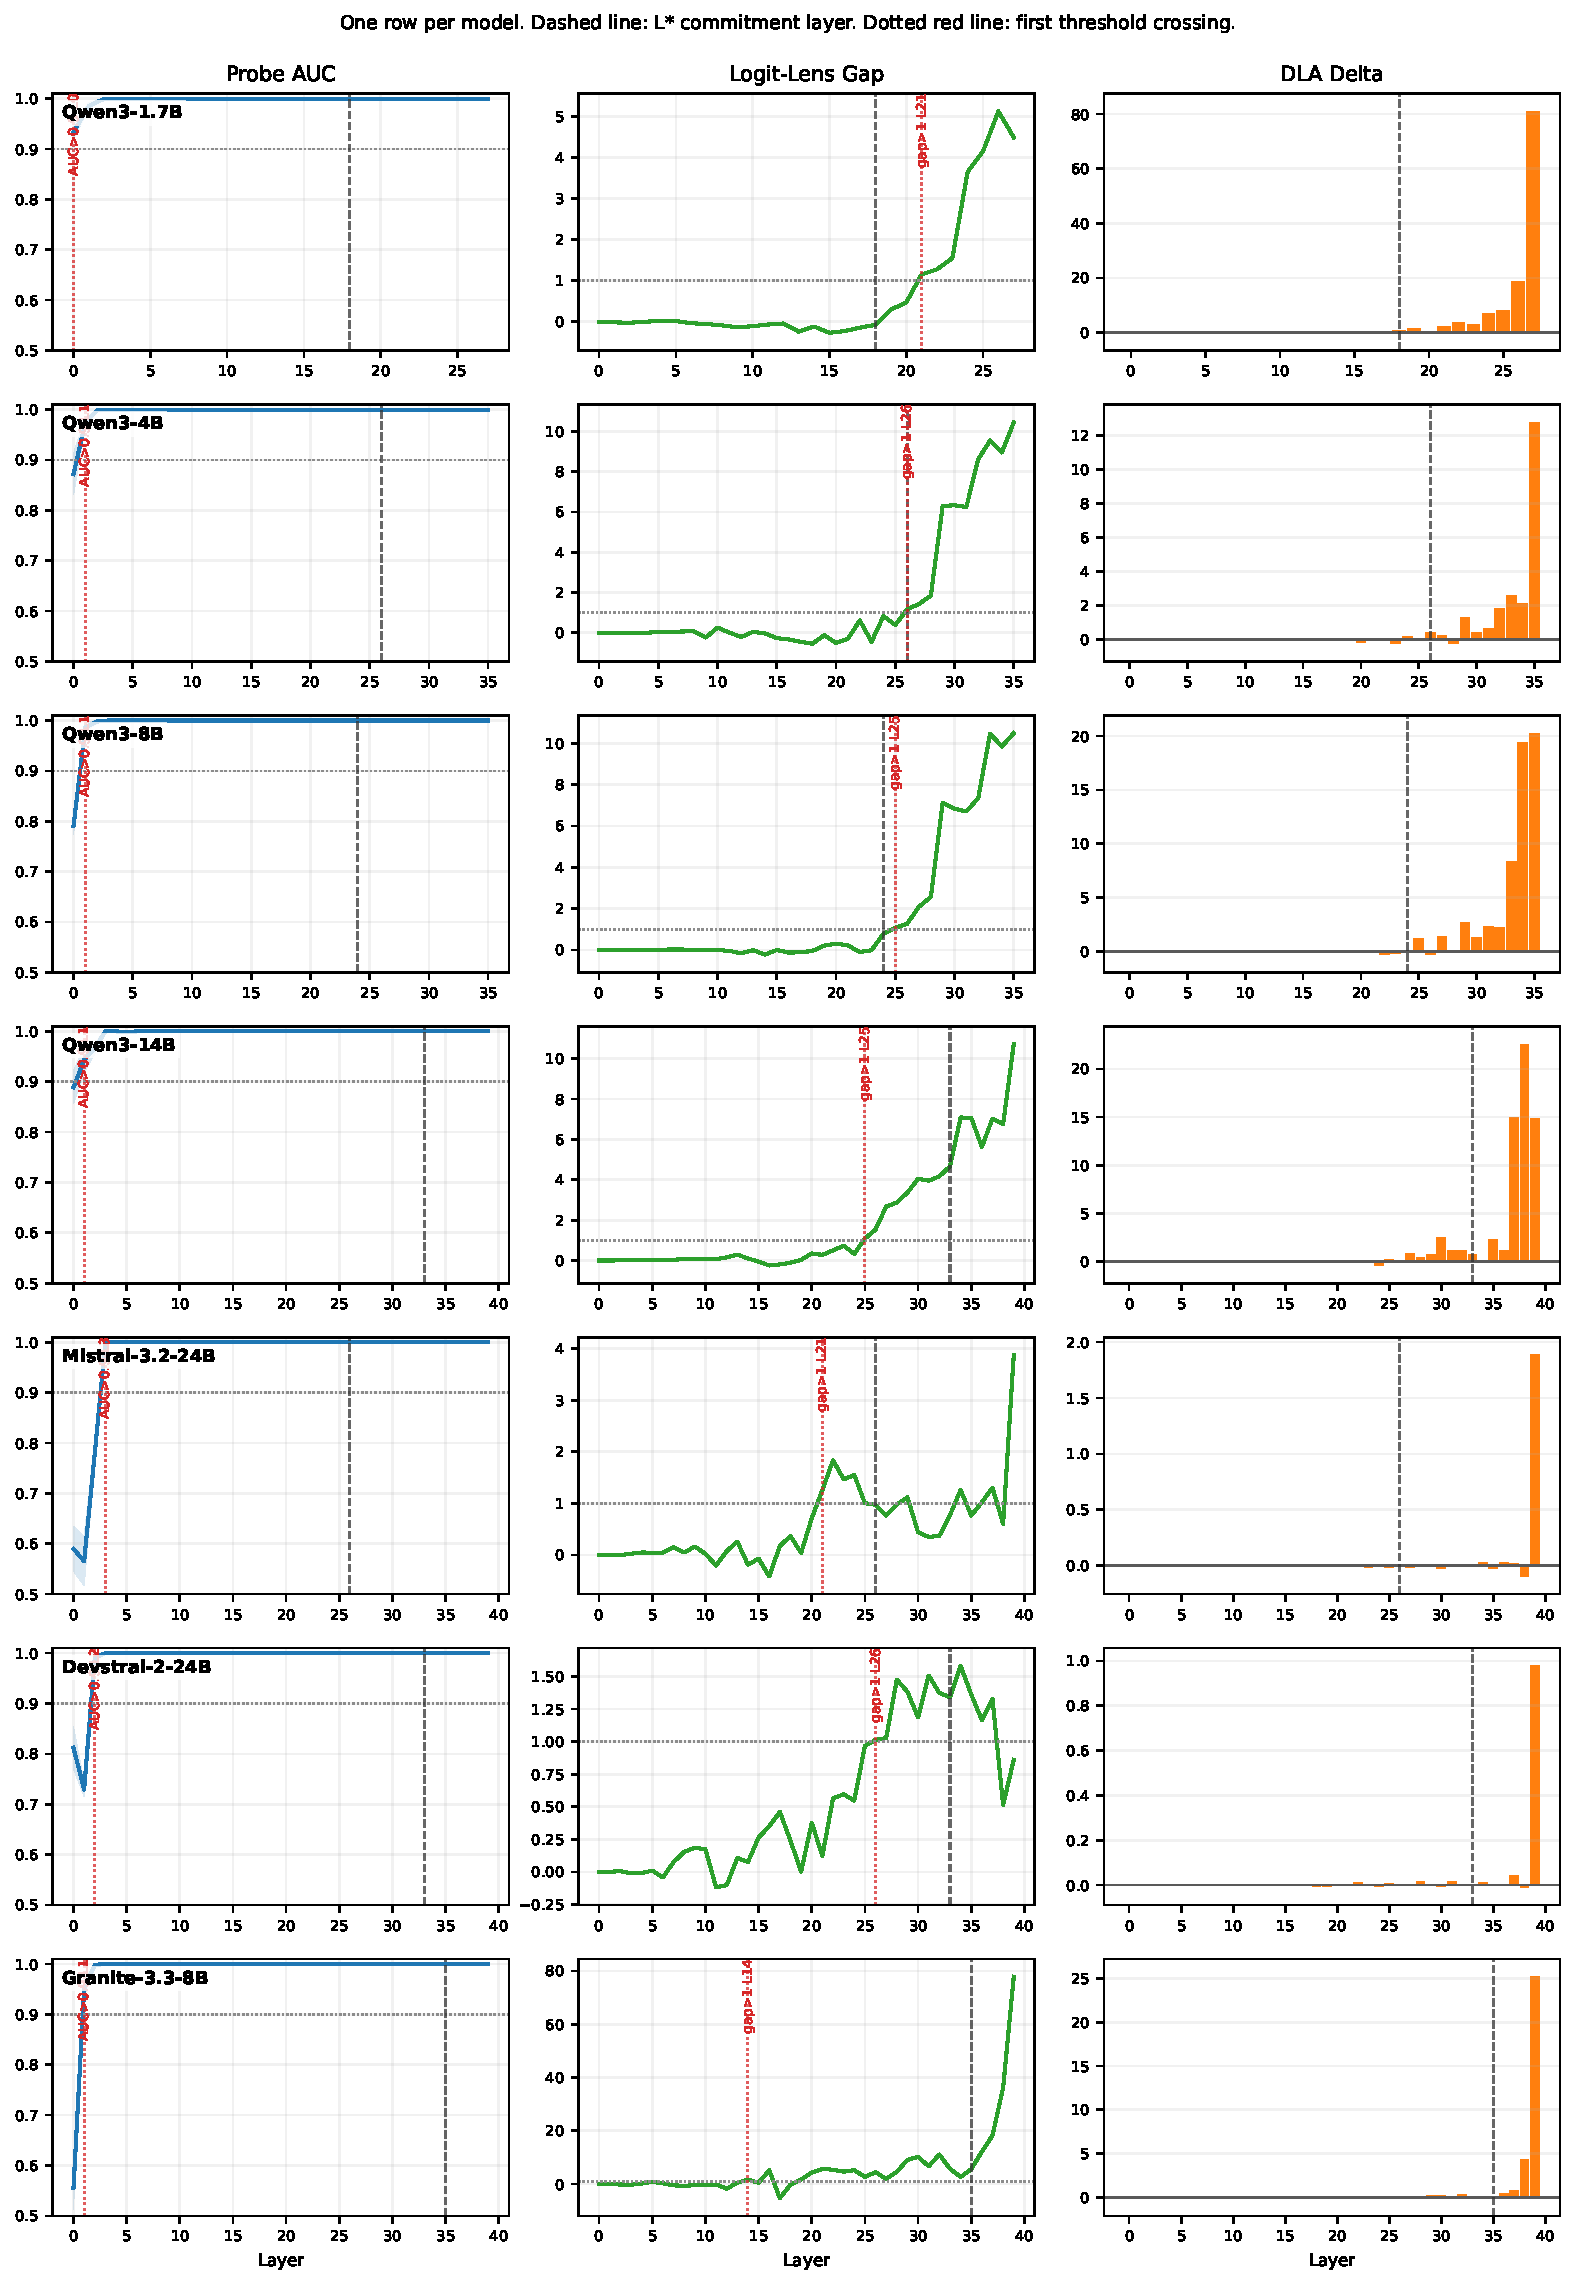
\includegraphics[width=\linewidth,height=0.84\textheight,keepaspectratio]{figures/triplet_allmodels.pdf}
  \caption{Triplet diagnostics across all seven models, arranged with one model
  per row and three diagnostics per row. From left to right, each row shows the
  linear probe AUC, the logit-lens clean-minus-corrupt gap, and the DLA sweep.
  All curves are computed on 300 held-out prompt pairs per model. Across
  families, probe separability appears early, whereas the causal
  logit-writing mass remains concentrated close to the top of the stack and
  near the commitment layer $L^*$. Granite is the clearest timing outlier: its
  logit-lens gap rises earlier than the other 40-layer models, but its largest
  DLA mass still sits in the final layers.}
  \label{fig:appendix-crossscale-triplet-curves}
\end{figure}

Figure~\ref{fig:appendix-crossscale-triplet-curves} makes the row-wise
comparison explicit.
\textbf{Qwen3-1.7B} already separates clean from corrupt prompts at L0, but its
logit-lens gap does not clear 1.0 until L21, and its strongest DLA writes are
the final three layers of the 28-layer stack.
\textbf{Qwen3-4B} and \textbf{Qwen3-8B} keep the same ordering, with probe
separability at L1, gap crossing only around L25--L26, and DLA concentrated in
L33--L35.
\textbf{Qwen3-14B} preserves the same shape in a deeper stack, with the late
readout pushed upward to L37--L39 around a later commitment layer L33.
\textbf{Mistral-Small-3.2-24B} still shows early-versus-late separation, but
its probe threshold arrives slightly later at L3 and its DLA is especially
concentrated in the final layer.
\textbf{Devstral-Small-2-24B} behaves similarly, with L2 probe separability,
L26 gap crossing, and a sparse late DLA pattern centered on L39.
\textbf{Granite-3.3-8B} is the main outlier in timing: the logit-lens gap
crosses 1.0 much earlier at L14, yet the dominant DLA writes still peak at
L39, L38, and L37. The cross-model regularity is therefore an ordering
statement---probe first, logit gap next, strongest direct writes last---rather
than an exact layer match across architectures.

\subsection{Scale-Specific Reader Identities}
\label{appendix:cross-scale:readers}

At every tested Qwen3 scale, the downstream readout structure is the same:
bridge heads redistribute attention to the tool schema, and a later structured
writer commits to the opening token. The specific component identities vary
with model size. The same attention-side schema reading pattern also appears in
the three non-Qwen models.

Table~\ref{tab:appendix-crossscale-readers} reports the formation-window write
ratio, the $K_{\mathrm{corrupt}}/K_{\mathrm{clean}}$ ratio when available, the
strongest schema-reading head, and the best-supported structured component per
model.
Values are drawn from Table~\ref{tab:crossscale} in the main text.

\begin{table}[h]
\centering
\small
\caption{Formation-window and readout component properties per model.
MLP/Attn is the ratio of $\hat{\mu}_\Delta$-direction write by MLP blocks
versus attention heads in the formation window. $K_{\mathrm{corrupt}}/K_{\mathrm{clean}}$
is the corrupt-higher versus clean-higher $|\kappa|$ mass ratio along $\hat{\mu}_\Delta$.
Best-head $\Delta$Attn is the clean-minus-corrupt attention shift for the
strongest schema-reading head. Key component is the most local named component
available from the follow-up analysis: a late feature when available, otherwise
the strongest later readout head from the upstream projection analysis.}
\label{tab:appendix-crossscale-readers}
\resizebox{\linewidth}{!}{%
\begin{tabular}{lccccc}
\toprule
Model & MLP/Attn & $K_{\mathrm{corrupt}}/K_{\mathrm{clean}}$ & Best-head $\Delta$Attn (pp) & Schema head & Key component \\
\midrule
Qwen3-1.7B & 3.39 & 261.2/163.1 & $+28.6$ & L21H1 & L27 F150019 \\
Qwen3-4B & 2.15 & 8.4/3.3 & $+69.0$ & L29H9 & L35 F14572 \\
Qwen3-8B & 2.75 & 24.4/10.9 & $+52.9$ & L29H9 & L34 F109925 \\
Qwen3-14B & 3.21 & 61.6/3.7 & $+72.6$ & L30H13 & L34H8 \\
Mistral-Small-3.2-24B & 1.49 & -- & $+8.8$ & L20H19 & L25H27 \\
Devstral-Small-2-24B & 2.70 & -- & $+37.3$ & L23H12 & L30H12 \\
Granite-3.3-8B & 2.45 & -- & $+25.2$ & L34H25 & L34H26 \\
\bottomrule
\end{tabular}
\hspace*{-0.2em}}
\par\vspace{0.3em}{\footnotesize Feature-level late-writer decompositions are
currently available only for the Qwen family. For the three non-Qwen rows,
$K_{\mathrm{corrupt}}/K_{\mathrm{clean}}$ remains unavailable without
Transcoder-based feature decomposition, and the key-component field therefore
uses the strongest later head from the upstream projection sweep as a coarse
readout proxy.}
\end{table}

At every Qwen3 scale, the MLP/Attn ratio exceeds 1.0 and
$K_{\mathrm{corrupt}}$ exceeds $K_{\mathrm{clean}}$, confirming that
MLP-dominated suppressor features account for most of the
$\hat{\mu}_\Delta$-direction write. The bridge head moves from L21H1 at 1.7B
to L29H9 at 4B and 8B, then to L30H13 at 14B. The same role split appears in
the additional families: an attention head reads the tool schema, while the
main causal mass remains MLP-heavy overall. In those three models the
best-supported later readout heads are L25H27 for Mistral, L30H12 for
Devstral, and L34H26 for Granite, distinct from the earlier schema-reading
heads listed in the same rows.

The abstract functional roles are shared across scales: the formation-window
MLPs write the suppression signal against the scaffold default, and the late
MLP block translates the resulting tool-call vector into the structural opening
token. The layer indices and specific feature identities shift with model
depth, but the computational logic is the same.

%% ------------------------------------------------------------
\section{Implementation Details}
\label{appendix:implementation}
%% ------------------------------------------------------------

\subsection{Transcoder Checkpoints}
\label{appendix:implementation:transcoder}

We use publicly released transcoder for Qwen3 from
\texttt{mwhanna/qwen3-8b-transcoders} (MIT license), which cover all 36 MLP
layers~\citep{dunefsky2024transcoders}.
Each transcoder maps from MLP pre-activations (\texttt{mlp.hook\_in}) to MLP
outputs (\texttt{mlp.hook\_out}) via a sparse encoder-decoder pair with ReLU
activations.
The feature dimension is $d_f = 163{,}840$, an expansion factor of $40{\times}$
over $d_{\mathrm{model}} = 4{,}096$.
Transcoders are trained with a sparsity regularization coefficient of 12
and a pre-activation penalty of $6 \times 10^{-5}$ for 122,070 steps at
batch size 8,192.

For the formation-window analysis we use layers L20--L23; for the late-MLP
readout analysis we use L34.
Feature semantic labels are assigned by inspecting (a) the top-activating
prompts from the 300 held-out pairs and (b) the top-weighted output tokens of
each decoder direction $w_f^{(\ell)}$.
Labeling is performed without reference to the $\kappa$ rankings to avoid
confirmation bias.

\subsection{Compute}
\label{appendix:implementation:compute}

All experiments use a single NVIDIA A6000 Pro GPU (96~GB VRAM).
Activation patching sweeps over all 36 layers and two token positions
on 300 prompt pairs require a single forward pass per (layer, position, prompt)
coordinate; the full sweep is batched and completes in under one GPU-hour.
The transcoder feature scoring over the formation window (L20--L23, 300 pairs)
takes approximately one GPU-hour, including the causal ablation runs.
The downstream readout sweep (L25--L35 DLA and single-component patching,
300 pairs) is the slowest 8B analysis because it evaluates every head and MLP
in the downstream window. Its exact wall-clock depends on batch size and
whether cached activations are reused, so we do not report a single stable
GPU-hour number here.
Cross-scale experiments (Qwen3-1.7B, 4B, 14B) follow the same protocol
on the same held-out set. Their wall-clock varies with model depth, hidden
width, and batching, so we likewise omit a single per-scale GPU-hour summary.
